\chapter{SAP APO System}
Das SAP \ac{APO} ist ein "`umfassendes  System, das im Rahmen der Supply Chain Initiative der SAP erstellt wurde (...). Es ist ein Werkzeugkasten für das Supply Chain Mangement (...)"' \cite[Abschnitt 4, Seite 5]{scm:script_17_1}. Es bietet eine vollständige integrierte Palette von Funktionen rund um die Planung und Ausführung von Logistikprozessen. Das SAP APO unterstützt die Punkte: \cite{scm:apo_2}
\begin{itemize}
	\item die unternehmensübergreifende Interaktion auf der strategischen, taktischen und operativen Planungsebene
	\item die Zusammenarbeit mit Logistikpartnern von der Auftragsannahme über die Bestandsüberwachung bis hin zum Produktversand
	\item die Pflege der Beziehungen sowohl zu Kunden als auch zu Geschäftspartnern
	\item die stetige Optimierung und Messung der Leistungsfähigkeit des Logistiknetzwerks
\end{itemize}

\section{Zusammenspiel zwischen SAP ERP und SAP APO}
Das SAP \ac{APO} System muss mit dem SAP \ac{ERP} System reibungslos zusammenspielen können. Dies ist notwendig, da das SAP \ac{APO} System auf die Daten des laufenden Geschäfts zugreifen muss, die wiederum im SAP ERP System anfallen. Darüber hinaus werden auch Stammdaten der Kunden, sämtliche Lieferanten, die Materialdaten der Produkte und die dazugehörigen Komponenten und auch die Stücklisten der herzustellenden Produkte definiert, gespeichert, verarbeitet und bereitgestellt. Auch die Bedarfsermittlung erfolgt im ERP System. Auf Basis dieser Werte werden die notwendigen Komponenten und Produkte beschafft oder hergestellt und eingelagert. Dazu gehören auch die Produktion mit Produktionsplanung und Produktionssteuerung, sowie der Vertrieb zum Umfang eines ERP-System. Darüber hinaus findet sich auch das Finanz- und Rechnungswesen als Modul in einem entsprechenden ERP-System. Kurz: ein ERP-System bildet die gesamte unternehmerische Tätigkeit in einem System ab.
Das \ac{APO}-System muss für die Planung und Deckung der Bedarfe auf diese Daten, in definierter Form zugreifen. Damit die Daten sauber ausgetauscht und vom SAO \ac{APO} sinnvoll integriert werden können, bedarf es einer standardisierten Schnittstelle, die die Daten verlässlich immer im selben Format liefert. Das SAP \ac{ERP} System stellt dazu das \ac{CIF} zur Verfügung. Über das \ac{CIF} werden die Daten  bidirektional über das Web ausgetauscht. Zusätzlich bietet das \ac{CIF} die folgenden Funktionen: \cite[Abschnitt 4.4, Seite 1 ff]{scm:script_17_1}
\begin{itemize}
	\item ein Integrationsmodell, das die Objekte definiert, die ausgetauscht werden
	\item einen Nachrichtenserialisierung, damit die Daten von beiden Seiten richtig gelesen werden 
	\item eine operative Datensicherung, die im Fehlerfall eingreift
	\item einen aktiven Datenkanal
	\item und einen Global Supply Chain Agent, der die Daten an die angeschlossenen System verteilt
\end{itemize}

\section{Module des SAP APO Systems}
Wie in \ref{fig:scm_komponent} zu sehen ist, gehören die folgenden Module zum SAP \ac{APO} System \cite[Abschnitt 4, Seite 6]{scm:script_17_1}
\begin{figure}[h]
	\centering
	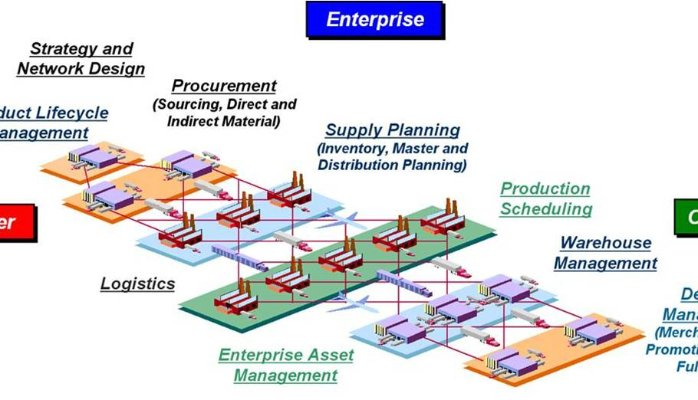
\includegraphics[width=0.8\textwidth]{../pics/scm_komponent}
	\caption{SAP APO Komponenten \cite{scm:grafik_scm_module_12}}
	\label{fig:scm_komponent}
\end{figure}

\begin{itemize}
	\item \ac{SCC}
	\item \ac{SCE}
	\item \ac{DP}
	\item \ac{SNP}
	\item \ac{TLB}
	\item \ac{PP/DS}
	\item \ac{ATP}
\end{itemize}

\begin{figure}[h]
	\centering
	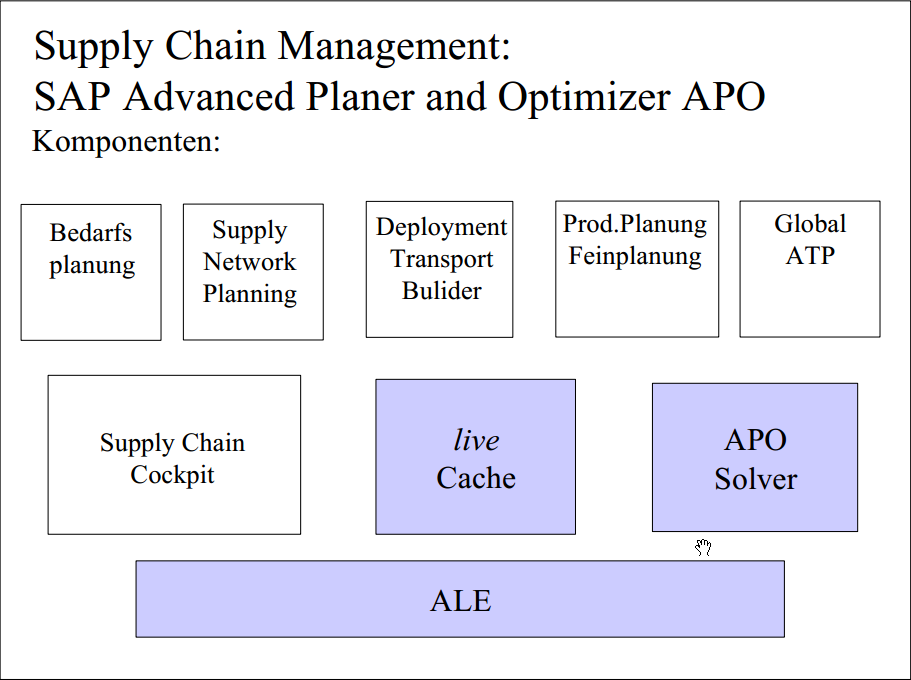
\includegraphics[width=0.8\textwidth]{../pics/scm_script_planungsmodi_APO-Module_nko}
	\caption{SAP APO Komponentenübersicht \cite[Abschnitt 4, Seite 6]{scm:script_17_1}}
	\label{fig:sap_apo_komp}
\end{figure}

Nachfolgend werden insbesondere die Komponenten \ac{DP}, \ac{SNP}, \ac{PP/DS}, \ac{ATP} und \ac{TLB} näher vorgestellt.

\subsection{Demand Planning}
Die \ac{DP} Komponente "`dient dazu, die Nachfrage nach verkaufsfähigen Produkten zu prognostizieren"'\cite[Abschnitt 4, Seite 12]{scm:script_17_1}. Das Ergebnis ist Absatzplan unter Berücksichtigung von Vergangenheitswerten aus dem \ac{ERP}-System oder InfoSources, wie beispielsweise Excel-Tabellen oder Business Warehouse.
Das Ziel eines erfolgreichen Unternehmens ist eine möglichst realitätsnahe Produktionsplanung anhand des Bedarfs aus der Vergangenheit. Das Problem ist, diese Prognose möglichst Präzise zu erarbeiten. Das liegt in erster Linie an der Unberechenbarkeit der Marktteilnehmer, also Handlungen der Konkurrenten und Konsumenten und deren Auswirkungen auf den Markt. Um dem entgegen zu wirken, wird eine möglichst umfangreiche Datenbasis benötigt, anhand der die Prognosen neu berechnet und an die geänderten Bedingungen angepasst werden. 
Zum Erstellen einer Prognose werden, im ersten Schritt, die Bedarfswerte vorangegangener Perioden benötigt. Mit Hilfe des \ac{DP} werden diese Daten analysiert und anschließend als zukünftiger Bedarf vorhergesagt. Typischerweise erhält man die Daten aus einem angrenzenden \ac{ERP}-System. Alternativ kann man über eine manuelle Eingabe, eigene Daten bereitstellen. Dem SAP \ac{APO} System stehen unter anderem die Modelle
\begin{itemize}
	\item \textit{Konstantmodell}
	\item \textit{Trendmodell}
	\item \textit{Lineare Regression }
	\item \textit{Saison- oder Trendsaisonmodell}
	\item \textit{Saison + lineare Regression}
\end{itemize}
als Prognosemodelle zur Verfügung. Mittels einer \textbf{automatischen} Methodenauswahl, wird anhand einer Reihe von Tests, die Methode gewählt, die die beste Prognose erstellt hätte. \cite[Abschnitt 4, Seite 14]{scm:script_17_1}
Bei den in \ref{fig:absatzzahlen} gezeigten Absatzzahlen handelt es sich um fiktive Vergangenheitswerte, die bei der Methodenauswahl und für die Erstellung eines Prognosemodells verwendet wurden. Die Zahlen wurden willkürlich zusammengestellt, um mehrere Prognosemodelle testen zu kommen. 
Die Daten wurden manuell anhand einer CSV-Datei in das SAP System eingelesen und anschließend in ein InfoCube geladen und gespeichert. Für reale oder echte Prognosen, werden stets kurze Zeiträume betrachtet. Dabei handelt es sich um einen kontinuierlichen Prozess bei dem neue Werte in das System importiert werden und ein erneutes berechnen der Prognose ansteuern. Dadurch soll die Prognose über einen längeren Zeitraum hinweg präzise bleiben. Im Folgenden werden die einzelnen Modelverfahren kurz vorgestellt.
\begin{figure}[h]
	\centering
	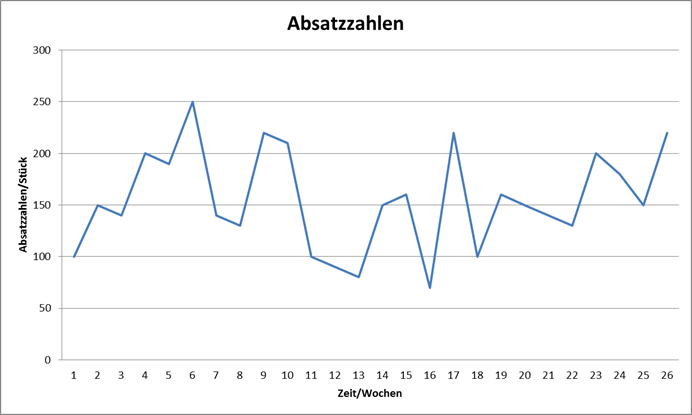
\includegraphics[width=0.8\textwidth]{../pics/absatzzahlen_nko}
	\caption{Fiktive Absatzzahlen}
	\label{fig:absatzzahlen}
\end{figure}
\subsubsection{Konstantmodell}
Das Konstantmodell erstellt eine Prognose auf dem gleitenden Mittelwert einer exponentiellen Glättung der ersten Ordnung \cite[ Abschnitt 4, Seite 14]{scm:script_17_1}. Für die Berechnung des Prognosewertes wird der letzte Vergangenheitswert mit dem vorhergehenden Prognosewerte und einem Glättungsfaktor \textit{Aplha} verrechnet. Der Glättungsfaktor Alpha ist für die Gewichtung der Vergangenheitswerte verantwortlich und berücksichtigt die aktuelleren Daten stärker, womit diese einen größeren Einfluss auf die \textit{neue} Prognose haben. 
Für Alpha wird ein Wert zwischen 0 und 1 gewählt. Bei einem Wert von 0 werden die errechneten Grundwerte beibehalten, was zur Folge hat, dass neuere Werte keinen Einfluss mehr auf die Prognose nehmen. Dementsprechend ist bei einem Wert von 1, entspricht der Durchschnittswert dem letzten Wert der Zeitreihe. Je nachdem ob die neuen Werte einen größeren Einfluss haben sollen, wählt man einen höheren Alpha Wert. Bei einem Wert von 0,5 beispielsweise, werden die Vergangenheitswerte folgendermaßen gewichtet \cite{scm:constmodel_3}:
\begin{enumerate}
	\item Erster oder aktuellster Vergangenheitswert: 50\%
	\item Zweiter Vergangenheitswert: 25\%
	\item Dritter Vergangenheitswert: 12,5\%
	\item Vierter Vergangenheitswert: 6,25\%
\end{enumerate}

Der Glättungsfaktor wird somit je Periode um die Hälfte des Wertes reduziert. Ein großer Wert verliert berücksichtigt somit die aktuellen Daten stärker. Typischerweise, sollen aber Zufälle oder Schwankungen ausgeglichen werden. Daher bietet sich ein Wert  kleiner als 0,5 an.
Die \ref{fig:konst_03} zeigt das Ergebnis einer Prognose des Konstantmodells mit einem Alpha Wert von 0,3. In der Abbildung lässt sich das Problem des Konstantmodells erkennen: die Vergangenheitswerte werden nicht richtig fortgeführt. Das liegt daran, dass das Kontantmodell eher für die Verwendung von Werten gedacht ist, die sehr geringe Schwankungen aufweisen. Das Ergebnis ist eine Gerade, beziehungsweise eine konstante Linie parallel zur X-Achse. Da das Konstantmodell eher "`für Zeitreihen, die keinen trendförmigen Verlauf aufweisen"' \cite{scm:constmodel_3} anwendbar ist und wir zu starke Schwankungen aufweisen, würde auch das Anpassen des Alpha-Wertes die Prognose nicht ändern.

\begin{figure}[h]
	\centering
	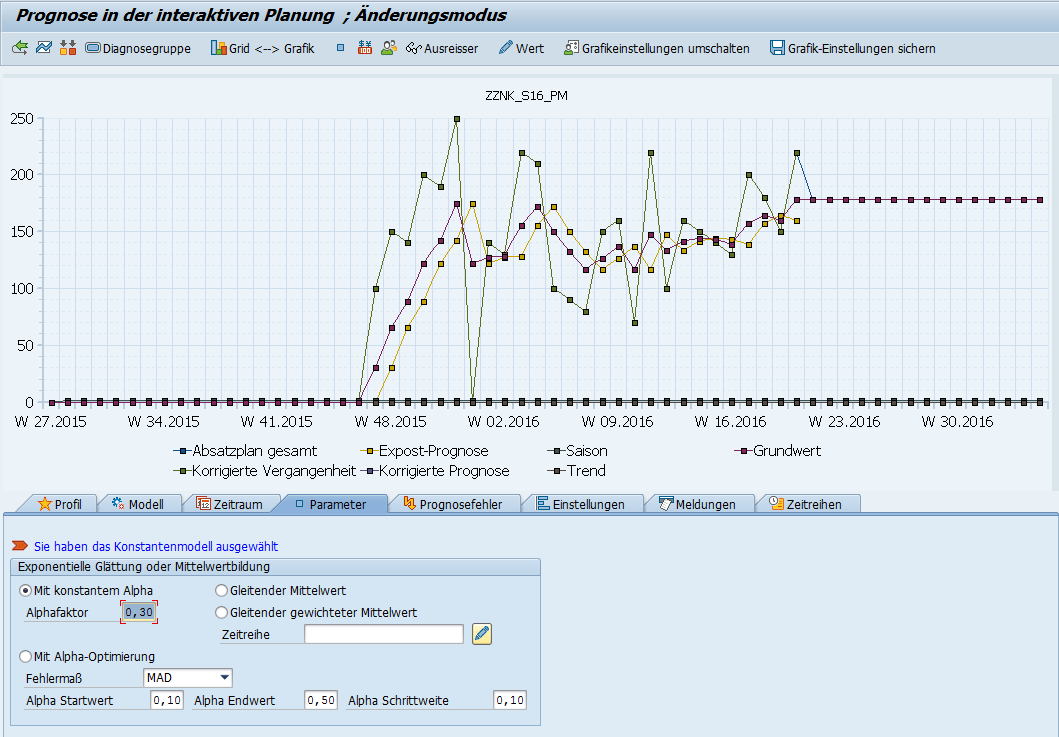
\includegraphics[width=0.8\textwidth]{../pics/Konstantmodell_nko}
	\caption{Prognosewert im Kontantmodell mit Alpha Wert 0,3}
	\label{fig:konst_03}
\end{figure}


Wie \ref{fig:konst_09} zeigt, sehen wir stattdessen, wie stark die Auswirkungen des vorhergehenden Vergangenheitswertes auf die Prognose ist und das die Gerade auf Höhe des letzten Vergangenheitswertes fortgeführt wird. In diesem konkreten Fall bilden wir lediglich den Bedarf nach.

\begin{figure}[h]
	\centering
	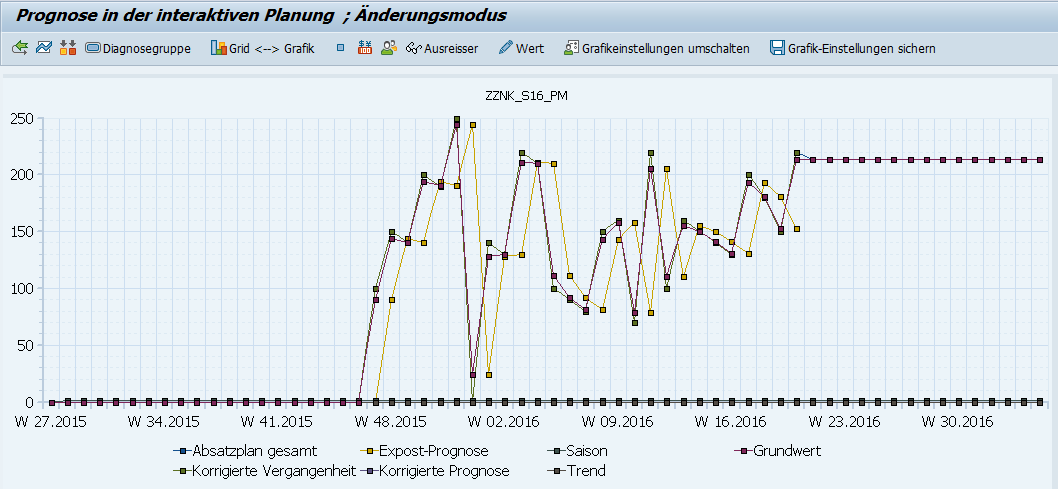
\includegraphics[width=0.8\textwidth]{../pics/Konstantmodell_nko_a_0_9}
	\caption{Prognosewert im Kontantmodell mit Alpha Wert 0,9}
	\label{fig:konst_09}
\end{figure}


\subsubsection{Trendmodell}
Als mögliche Alternative zum Konstantmodell bietet sich das Trendmodell an. Ein Trendmodell berücksichtigt Trends und kann diese entsprechend in den Prognosewerten abbilden. Für die Berechnungen liegt dem Trendmodell "`die exponentielle Glättung 2. Ordnung"'\cite[Abschnitt 4, Seite 14]{scm:script_17_1}. Für die Vorhersagewerte wird zuerst die Formel der ersten exponentiellen Glättung angewandt und anschließend wird das Ergebnis nochmal geglättet. \cite{scm:second_order_exp_4} Analog zum Konstantmodell wird auch beim Trendmodell der Alpha Faktor, mit der gleichen Funktionalität, berücksichtigt. Die \ref{fig:trend} zeigt die Prognosewerte mit den fiktiven Beispielwerten. Anders als das Konstantmodell werden hier Trends erkannt und fortgeführt, wodurch dieses Model geeigneter ist um Prognosen zu erstellen.

\begin{figure}[h]
	\centering
	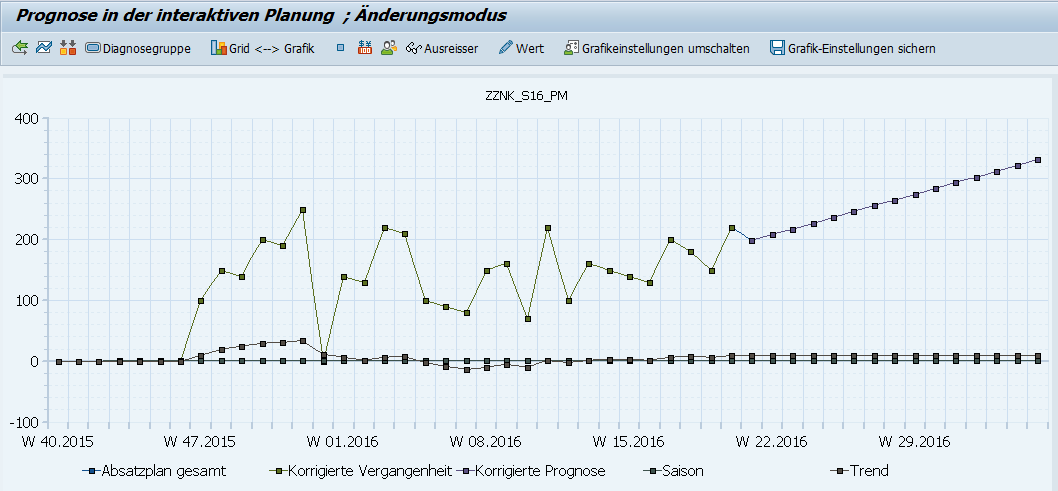
\includegraphics[width=0.8\textwidth]{../pics/Trendmodell_nko}
	\caption{Prognosewert im Trendmodell}
	\label{fig:trend}
\end{figure}

\subsubsection{Lineares Regressionsmodell}
Ähnlich wie Trendmodelle, werden auch Regressionsmodelle für die Vorhersage von Trends verwendet. Dabei handelt es sich um eine statistische Methode, die eine Gerade, basierend auf den Vergangenheitswerten bestimmt. Dabei soll die Gerade den Abstand zwischen den Vergangenheitswerten minimal halten. Anders als bei den anderen Methoden werden die Vorhersageparameter nicht durch vorhergehende Annahmen beeinflusst um anschließend die Prognose von Periode zu Periode zu verbessern. \cite{scm:lin_reg_5}
Die \ref{fig:lin_reg} zeigt das Ergebnis der linearen Regressionsmethode. 

\begin{figure}[h]
	\centering
	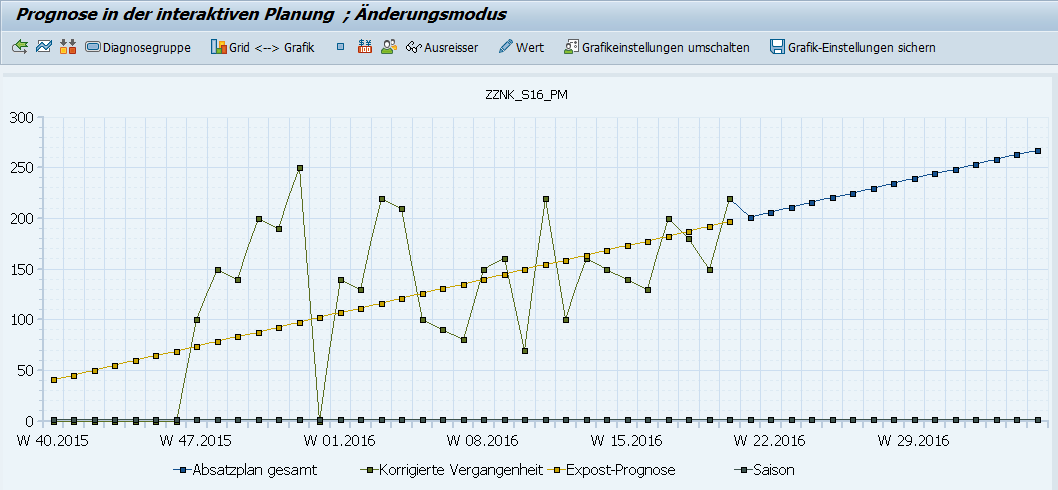
\includegraphics[width=0.8\textwidth]{../pics/Lineare_Regressionmodell_nko}
	\caption{Prognosewerte des linearen Regressionsmodells}
	\label{fig:lin_reg}
\end{figure}
Da die lineare Regression zwar einen Trend erkennen lässt und diesen fortführt, aber saisonal Schwankungen außer Acht lässt, ist auch diese Methode für unsere fiktiven Zahlen nicht geeignet.

\subsubsection{Saisonmodell}
Beim Saisonmodell handelt es sich um ein Trendmodell, das auch saisonale Schwankungen erfasst und diese mit in die Prognose aufnimmt. Dieses Modell wird typischerweise für die Berechnung von Zeitreihen verwendet, die zusätzlich saisonal Daten enthalten. Analog zum Konstanten- oder Trendmodell, wird ein Alpha Wert gesetzt, um den Grundwert zu \textit{glätten}. Zusätzlich existiert ein Gamma-Wert, der die Saisonkomponente bestimmt. 
Wie in \ref{fig:saison} zu sehen ist, eignet sich das Saisonmodell besonders bei Daten, die saisonale Schwankungen beinhalten. Die Schwankung sollte jedoch keine allzu große Varianz aufweisen, da sonst das Ergebnis verfälscht wird. Ein weiteres Problem des Modells ist, dass es viele Vergangenheitswerte benötigt um sauber und für längere Perioden fortgeführt zu werden.
\begin{figure}[h]
	\centering
	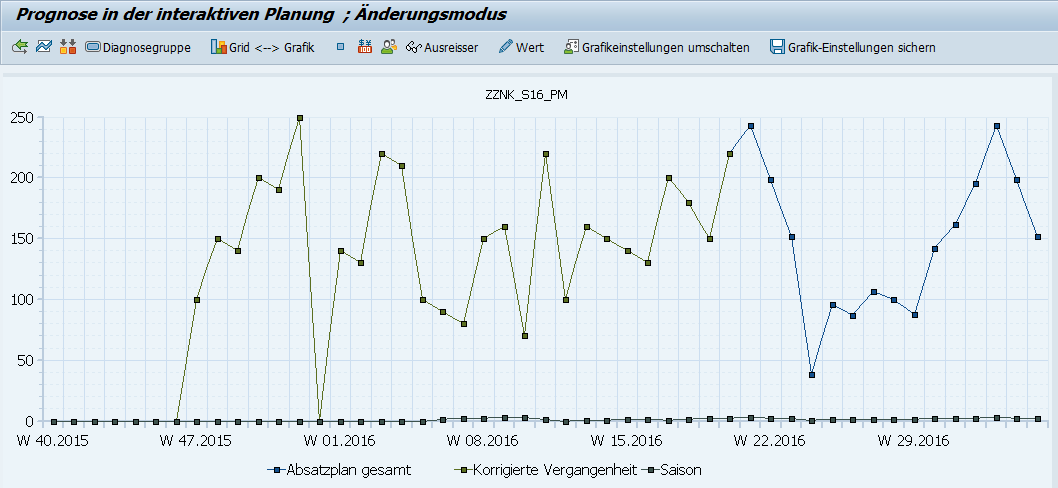
\includegraphics[width=0.8\textwidth]{../pics/Saisonmodell_nko}
	\caption{Prognosewert mit dem Saisonmodell}
	\label{fig:saison}
\end{figure}

\subsubsection{Saison + Lineares Regressionsmodell}
Beim Saison und Lineare Regressionsmodell wird zuerst ein Saisontest durchgeführt, um festzustellen ob die Vergangenheitsdaten eine saisonale Komponente enthalten und anschließend, sofern der Test erfolgreich ist, werden die Saisonindizes berechnet und die Prognosewerte bestimmt. Schlägt der Test fehl, weil keine saisonale Komponente vorhanden ist, so führt das Model eine lineare Regression durch. \cite{scm:season_lin_reg_6}
In \ref{fig:sais_lin_reg} sieht man das Ergebnis dieses Modells.

\begin{figure}[h]
	\centering
	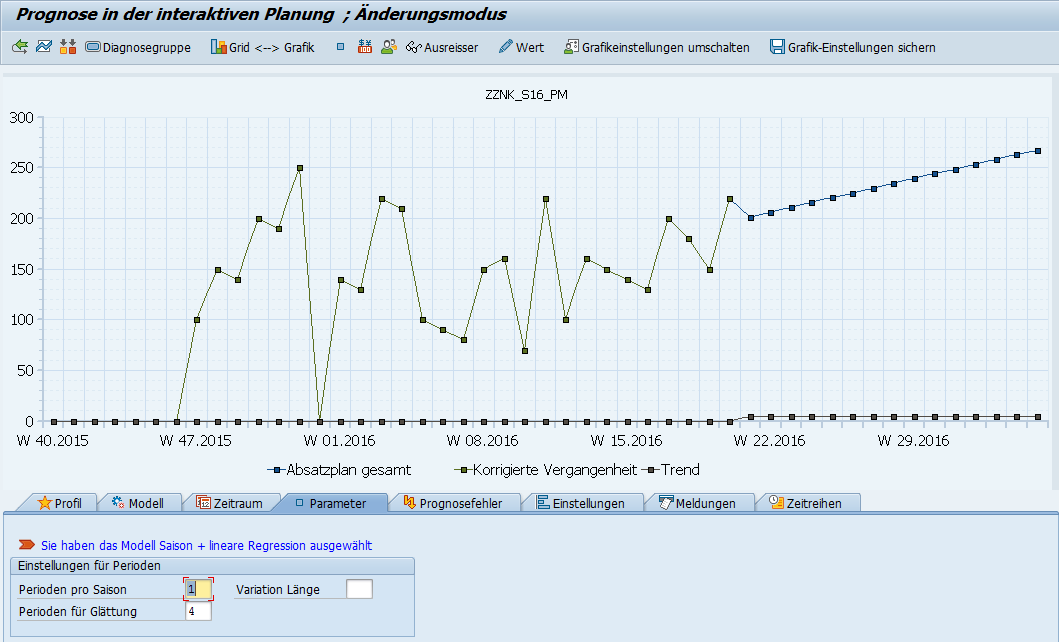
\includegraphics[width=0.8\textwidth]{../pics/lineare_sainsonal_regressionamodell_nko}
	\caption{Prognosewerte des Saison + lineare Regressionsmodells}
	\label{fig:sais_lin_reg}
\end{figure}
Ähnlich wie beim Saison-Model, existieren auch für dieses Modell nicht genug Vergangenheitswerte, um die saisonalen Schwankungen zu prognostizieren. 

\subsubsection{Trendsaisonmodell}
Beim Trendsaisonmodell werden zur Berechnung der Prognose sowohl ein Trend als auch saisonale Schwankungen berücksichtigt. Nach der Anfangsperiode werden sowohl der Grundwert, als auch der Trendwert und der Saisonindex berechnet. \cite{scm:trends_season_lin_reg_7}
die \ref{fig:trend_sais} zeigt das Ergebnis der Prognose mit dem Trendsaisonmodell. Mit den Glättungsfaktoren Alpha, Beta und Gamma werden Grundwert, Saisonindex  und Trendwert angepasst, um ein möglichst genau Prognose zu erhalten. 
Verglichen mit den anderen Modellen passt dieses Ergebnis am besten für die vorgegebenen Vergangenheitswerte. Die Expost-Prognose stimmt weitestgehend mit den Punkten des gesamten Absatzes überein. Ausgehend von den beliebig gewählten Vergangenheitswerten, führt die Prognose die gegebene Struktur fort.


\begin{figure}[h]
	\centering
	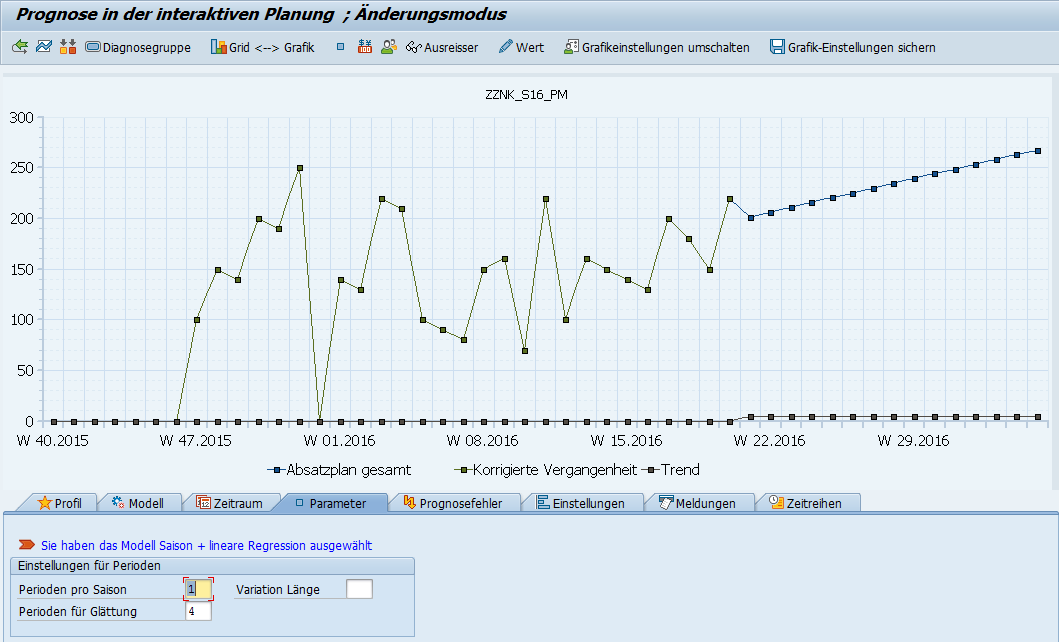
\includegraphics[width=0.8\textwidth]{../pics/lineare_sainsonal_regressionamodell_nko}
	\caption{Prognosewerte mit dem Trendsaisonmodell}
	\label{fig:trend_sais}
\end{figure}



\subsection{Supply Networt Planning}
Die Komponente \ac{SNP} ist verantwortlich für die Distributionsplanung, die Produktionsplanung und die Fremdbeschaffung. \cite[Abschnitt 4.3.4, Seite 1]{scm:script_17_1}
Nach der Wahl eines passenden Prognosemodells, wird darauf folgend die Produktion des prognostizierten Absatzes begonnen. Damit die Produktion beginnen kann muss jedoch der jeweilige Bedarf an Produktionsgütern beschafft werden. 
Die \ac{SNP} ermöglicht Simulationen und Umsetzungen von umfangreichen Planungsentscheidungen. Dabei wird, anhand von mathematischer Optimierungsverfahren und unter Berücksichtigung verschiedener \textit{Constraints} (Bedingungen), der Produktfluss entlang einer Logistikkette geplant. "`Das Ziel sind optimale Beschaffungs-,  Distributions- und Produktionsentscheidungen; Reduktion von Bestellabwicklungszeiten und Lagerbeständen; und ein verbesserter Kundenservice“'\cite{scm:snp_8}.
Gerade die Constraints spielen eine wichtige Rolle. Das Hauptziel von Constraints ist die Berücksichtigung von realen  Bedingungen, wie beispielsweise beschränkte Kapazitäten. Dazu gehören \cite[Abschnitt 4.3.4, Seite 1 f]{scm:script_17_1}
\begin{itemize}
	\item Transportbeschränkungen mittels Flugzeug, Frachter, Zug oder LWK, da nur bestimmte Mengen transportiert werden, 
	\item Lagerkapazitäten, weil ein Lager nur eine bestimmte Menge aufnehmen kann und 
	\item Fertigungskapazitäten, weil nur eine bestimmte Menge zu einer bestimmten Zeit produziert werden kann.
\end{itemize}

Durch die Berücksichtigung dieser Beschränkungen "`sind die Planungsergebnisse weit besser, als sie im herkömmlichen \ac{ERP}-System sein können“' \cite[Abschnitt 4.3.4, Seite 1 f]{scm:script_17_1}
Basierend auf dem Absatzplan der \ac{DP}-Komponente, plant die \ac{SNP}-Komponente die optimale Bedarfsdeckung und berücksichtigt die ganze \ac{SC}. Der \ac{SNP} erstellt die Plannung „auf aggregierten Bucket-Ressourcen“ \cite[Abschnitt 4.3.4, Seite 1]{scm:script_17_1}. Wobei sich die Größe des Buckets, an der zur Verfügung stehenden Kapazität anpasst. Somit wird festgestellt, ob ausreichend Kapazitäten vorhanden sind, um einen Bedarf zu befrieden und folglich fristgerecht produziert und geliefert werden kann. Jedoch werden bei der Planung nur die frei verfügbaren Kapazitäten berücksichtigt und nicht die optimale Produktionsreihenfolge.
Die nachfolgenden \ref{fig:snp_dist} und \ref{fig:snp_prod} zeigen den ermittelten Gesamtbedarf und -zugang im \ac{SNP}, nachdem die Netzwerkheuristik \cite[Abschnitt 4.3.4, Seite 7 f]{scm:script_17_1} durchgeführt wurde, die Distributionszugänge geplant und die Produktionsplanung ausgeführt wurde.
Die Pläne zeigen den benötigten Bedarf mit auf den Tag genauer Zuordnung und verdeutlichen, wann und wie viele Produkte produziert werden.

\begin{figure}[h]
	\centering
	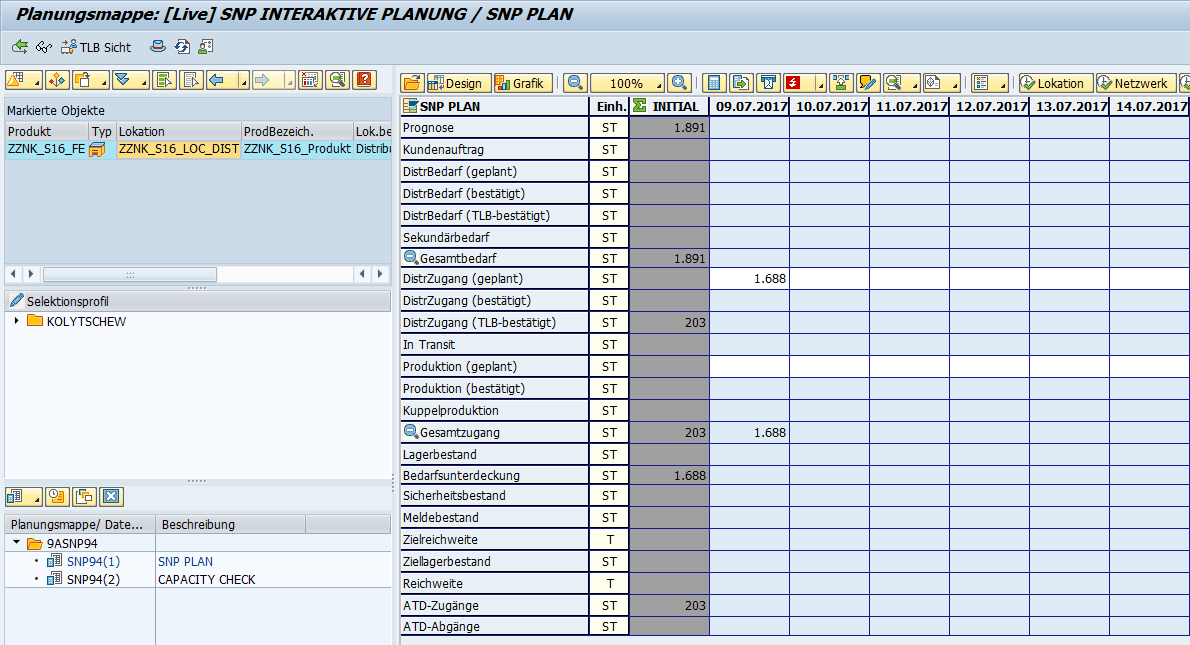
\includegraphics[width=0.8\textwidth]{../pics/SNP_dist_nko}
	\caption{SNP für das Distributionswerk}
	\label{fig:snp_dist}
\end{figure}

\begin{figure}[h]
	\centering
	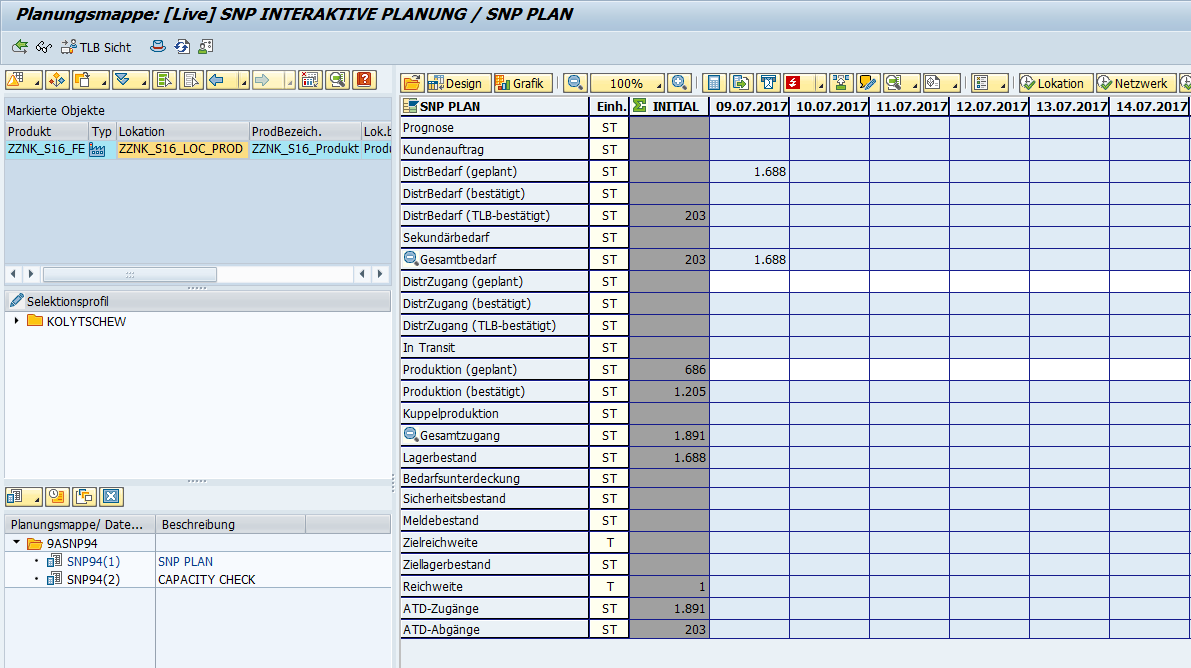
\includegraphics[width=0.8\textwidth]{../pics/SNP_prod_nko}
	\caption{SNP für das Produktionswerk}
	\label{fig:snp_prod}
\end{figure}

\subsection{Transport Load Builder}
Nachdem Abschluss des \ac{SNP} werden die optimale Transportladung der Transportmittel zusammengestellt. 
Der \ac{TLB} führt die Aufträge, die sich aus dem \ac{SNP} ergeben haben, in Transportaufträge und berücksichtigt dabei \cite[Abschnitt 4.3.4, Seite 5]{scm:script_17_1}
\begin{itemize}
	\item die verschiedenen Transportmittel, die damit transportierten Produkte und die verbundenen Transportkosten
	\item das minimale und maximal zulässige Gewicht der Transportladungen
	\item die maximale Anzahl an Transportpaletten je Transport und das maximale Volumen je Transportmittel.
\end{itemize}

Ziel der Komponenten ist, dass die Transportmittel möglichst ausgelastet sind. Daher spielt neben der Kapazität auch die Tauglichkeit des Transportmittels für ein Produkt eine Rolle. Abschließend müssen auch die wirtschaftlichen Aspekte berücksichtigt werden. Dazu werden die entsprechenden Transportkosten des Transportmittels und die Menge des zu transportierenden Produktes verglichen.

\subsection{Production Planning and Detailed Scheduling}
Nachdem die optimale Nutzung der Transportmittel feststeht, wird die Produktionsplanung durchgeführt. Dazu wird \ac{APO}-Komponente \ac{PP/DS} verwendet, welche die Ergebnisse aus dem \ac{SNP} nimmt und verfeinert.
Die Komponente hat einige Überschneidungen mit "`der SAP R/3 Komponente PP, [geht] in seinen Möglichkeiten jedoch deutlich darüber hinaus“' \cite[Abschnitt 4.3.4, Seite 11]{scm:script_17_1}. 
Für die Produktions- und Feinplanung verfeinert die \ac{PP/DS} Komponente die Planungsergebnisse aus der \ac{SNP}-Komponente. Die resultierenden Produktionspläne können minuten- oder sekundengenau sein. Dabei werden auch die Verfügbarkeit von Komponenten und Ressourcen berücksichtigt. Da die \ac{PP/DS} Komponente detailliertere Randbedienungen als das \ac{SNP} berücksichtigt, reduziert sich der Vorhersagezeitraum. Die Ergebnisse des \ac{PP/DS} gehen nicht so weit in die Zukunft, wie der Plan des \ac{SNP}. \cite[Abschnitt 4.3.4, Seite 11]{scm:script_17_1}
Ein optimaler Produktionsplan muss individuell an die Strategie und Bedürfnisse des Unternehmens und des Produkts angepasst werden. Darüber hinaus muss sich die Planungsrichtung (vorwärts, beziehungsweise rückwärts) bestimmen und anpassen lassen. Das bedeutet auch, dass bei der Strategie \textit{Rückwärts mit Umkehr} die Komponente auch, beziehungsweise primär in der Vergangenheit nach Möglichkeiten sucht einen Auftrag einzuplanen und erst, wenn die Sucher erfolglos ist, also keine Kapazitäten verfügbar sind, wird in der Zukunft nach freien Kapazitäten gesucht.
Im Planungsmodus wird festgelegt, auf welches Art und Weise das System die ausgewählten Ressourcen ein-, beziehungsweise um plant. Dabei stehen unter anderem die folgenden finiten und infiniten Planungsmodi zur Verfügung: \cite[Abschnitt 4.3.4, Seite 11f]{scm:script_17_1}\cite{scm:planungsmode_9}
\begin{itemize}
	\item Finiter Planen
	\item Lücke suchen
	\item Vorgang einfügen
	\item Vorgang einrütteln
\end{itemize}
Beim finiten Planen – Planungsmodus wird versucht die Aufträge entsprechend eines Endtermins, beispielsweise aktuelles Datum, frühester Endtermin oder spezifizierter Termin an dem der Auftrag fertig sein soll, einzuplanen, ohne bestehenden Ressourcenbelegungen zu berücksichtigen. 
Bei der infiniten Reihenfolgenplanung wird versucht, die Aufträge nacheinander abzuarbeiten. Beim Planungsmodus \textit{Lücke suchen} wird nach einer Lücke gesucht, die groß genug ist, um den Auftrag einzuplanen. Beim Planungsmodus \textit{Vorgang einfügen} versucht das System den Vorgang möglichst nah am vorgeschlagenen Termin einzufügen. Beim Modus \textit{Vorgang einrütteln} wird ebenfalls versucht den Auftrag möglichst nah am vorgeschlagenen Termin einzufügen. Falls die \textit{Lücke} für den Auftrag zu klein ist, werden die umliegenden Vorgänge so verschoben, dass die Lücke anschließend ausreicht. Die \ref{fig:planungsmodi} visualisiert die einzelnen Vorgänge.

\begin{figure}[h]
	\centering
	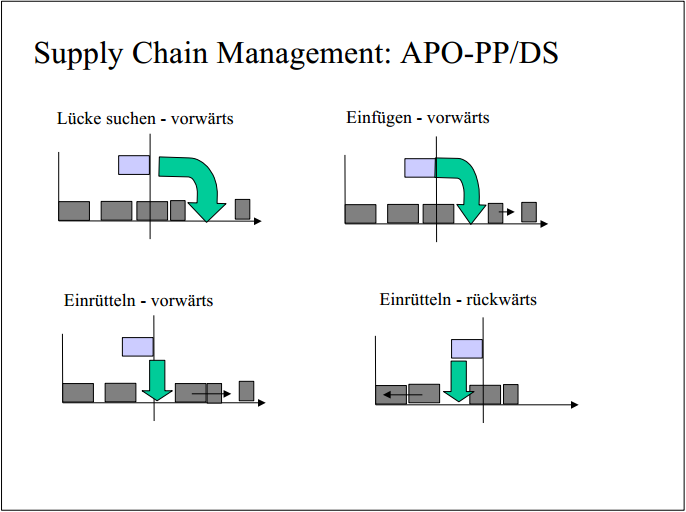
\includegraphics[width=0.8\textwidth]{../pics/scm_script_planungsmodi_finit_nko}
	\caption{Finite Planungsmodi \cite[Abschnitt 4.3.4, Seite 12]{scm:script_17_1}}
	\label{fig:planungsmodi}
\end{figure}

Abschließend wird die \textbf{Pegging-Beziehung} festgelegt. Dabei wird die Beziehung zwischen Bedarf und Vorgang definiert. Dabei wird zwischen dynamischen oder fixen Pegging unterschieden. Beim dynamischen Pegging passt das System die Zuordnung dynamisch an den Produktionsplan an. Beim fixen Pegging wird genau definiert, "`welcher Bedarf durch welches Angebot gedeckt wird“'. \cite[Abschnitt 4.3.4, Seite 12]{scm:script_17_1}
Die \ref{fig:planversion} zeigt die Zugangssicht zu unserem \ac{SNP}. Hier können wir einen Planungsautrag setzten.

\begin{figure}[h]
	\centering
	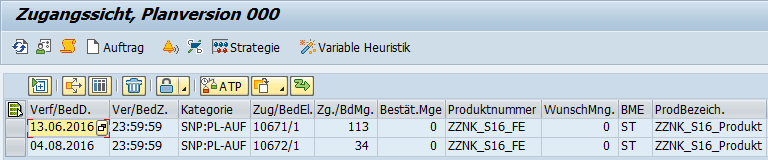
\includegraphics[width=0.8\textwidth]{../pics/PPDS_zugangssicht_nko}
	\caption{PP/DS Zugangssicht}
	\label{fig:planversion}
\end{figure}

\ref{fig:pplanung} stellt die Produktsicht und das Ergebnis der \ac{PP/DS} dar. Es werden hier die Informationen zu Bedarf, zu den Zugängen, sowie den Beständen im Produktionswerk dargestellt. Dabei wurden hier bereits die Strategieentscheidungen, die in den vorhergehenden Abschnitten erläutern wurden, berücksichtigt.

\begin{figure}[h]
	\centering
	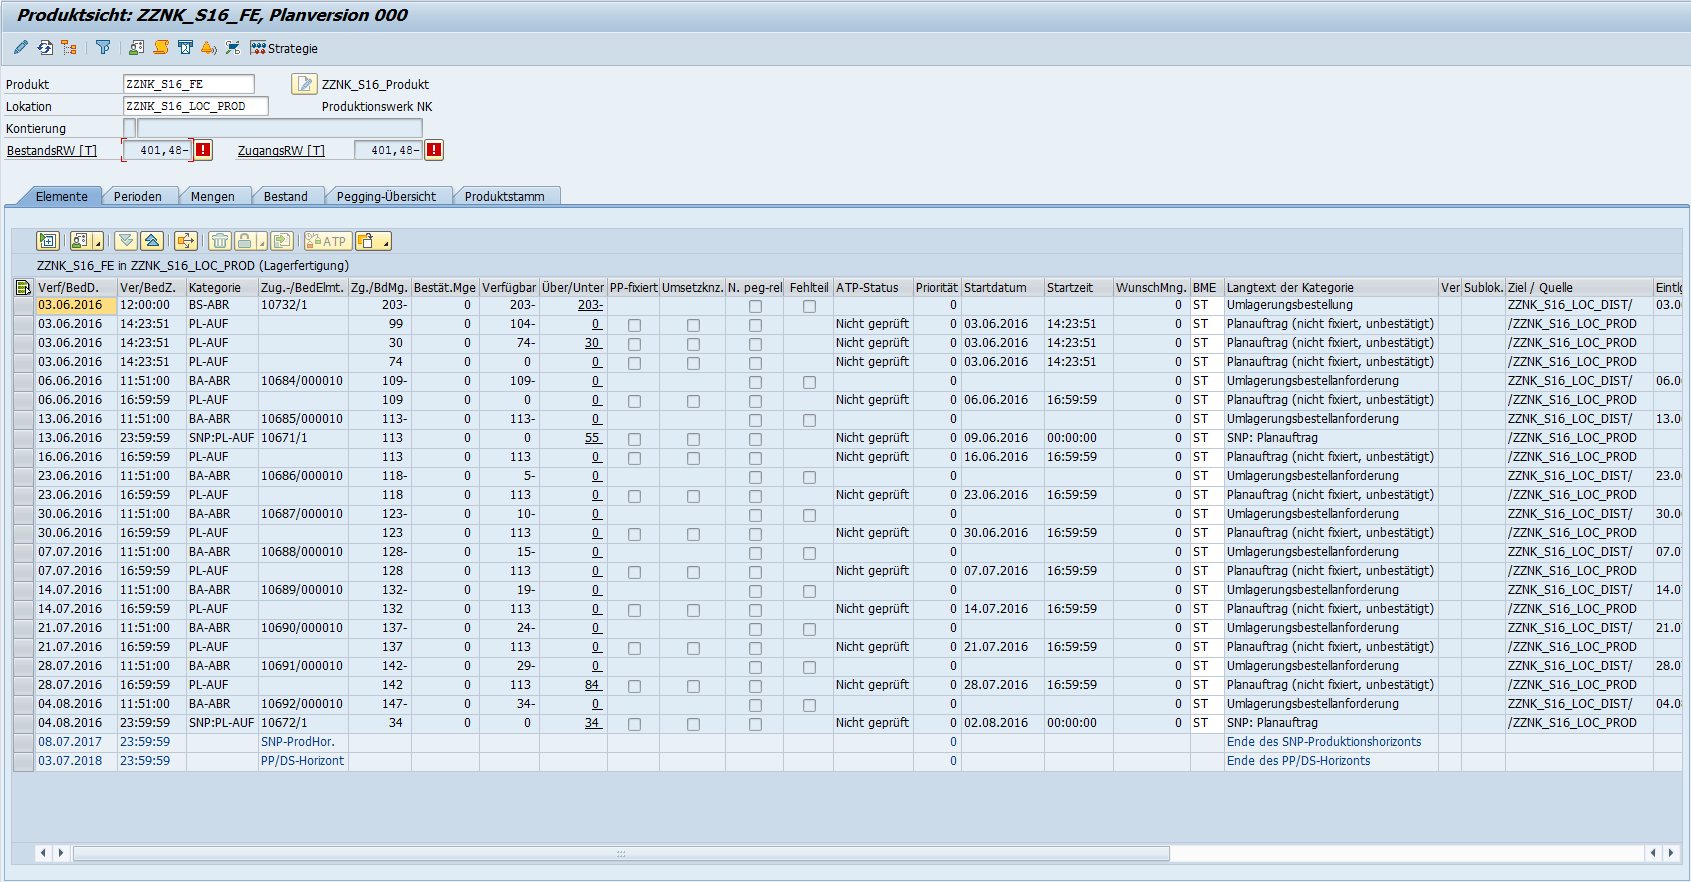
\includegraphics[width=0.8\textwidth]{../pics/Produktsicht_nko}
	\caption{Produktsicht mit Planauftrag}
	\label{fig:pplanung}
\end{figure}
In der Produktplantafel sind die möglichen freien Kapazitäten sichtbar. Nachdem die Aufträge eingeplant wurden, sollten keine freien Kapazitäten mehr verfügbar sein.

\subsection{Global Available-to-Promise}
Nachdem nun auch die Produktionspläne erstellt und die Kapazitäten verplant wurden, soll im nächsten Schritt die Verfügbarkeitsprüfung durchgeführt werden. 
Die \ac{ATP} Komponente überprüft die globale Verfügbarkeit der benötigten Ressourcen. Dabei werden nicht nur die aktuellen Bestände betrachtete, sondern auch sämtliche geplanten Zugänge, sowohl aus eigener Produktion als auch über Fremdbeschaffung. Durch die Zusammenarbeit mit mehreren \ac{ERP}-Systemen, lässt sich eine Verfügbarkeitsprüfung entlang der \ac{SC}, auch über mehrere Unternehmen hinweg, durchführen. Dadurch lässt sich feststellen, "`ob das gesuchte Produkt in der gesuchten Menge zum gewünscht Zeitpunkt verfügbar sein kann“'. \cite[Abschnitt 4.3.4, Seite 18]{scm:script_17_1}
Bei der Verfügbarkeitsprüfung lasst sich verschiedene Regeln festlegen, anhand deren beispielsweise zuerst überprüft wird, ob das Produkt im eigenen Lager vorhanden ist. Falls das Produkt nicht im Lager vorhanden ist, soll nach einem adäquaten Ersatzprodukt gesucht werden. Sollte auch diese Suche ohne Ergebnis verlaufen, wird die Suche in einem Lager an einem anderen Standort wiederholt und erneut geprüft ob entweder das Produkt oder ein adäquates Ersatzprodukt vorhanden ist und zum Produktionswerk versendet werden kann. Abschließend wird kontrolliert, ob das Produkt insgesamt hergestellt werden kann. Dafür müssen alle notwendigen Einzelteile im Lager zur Verfügung stehen. Falls das nicht zutrifft, wird erneut geprüft, wo und wie die fehlenden Komponenten beschafft werden. \cite[Abschnitt 4.3.4, Seite 18 f]{scm:script_17_1}
Da Produkte aus multiplen Komponenten bestehen und auch diese aus weiteren Komponenten bestehen können, kann eine Komponenten- oder Kapazitätsprüfung zu Performance Problemen führen, da das \ac{APO}-System auf das entsprechenden \ac{ERP}-System zugreifen muss. Um dem entgegen zu wirken bietet es sich an, die für die Verfügbarkeitsprüfung relevanten Daten, im Speicher des APO-Systems zu halten und zur Verfügung zu stellen.

